
% Default to the notebook output style

    


% Inherit from the specified cell style.




    
\documentclass[11pt]{article}

    
    
    \usepackage[T1]{fontenc}
    % Nicer default font (+ math font) than Computer Modern for most use cases
    \usepackage{mathpazo}

    % Basic figure setup, for now with no caption control since it's done
    % automatically by Pandoc (which extracts ![](path) syntax from Markdown).
    \usepackage{graphicx}
    % We will generate all images so they have a width \maxwidth. This means
    % that they will get their normal width if they fit onto the page, but
    % are scaled down if they would overflow the margins.
    \makeatletter
    \def\maxwidth{\ifdim\Gin@nat@width>\linewidth\linewidth
    \else\Gin@nat@width\fi}
    \makeatother
    \let\Oldincludegraphics\includegraphics
    % Set max figure width to be 80% of text width, for now hardcoded.
    \renewcommand{\includegraphics}[1]{\Oldincludegraphics[width=.8\maxwidth]{#1}}
    % Ensure that by default, figures have no caption (until we provide a
    % proper Figure object with a Caption API and a way to capture that
    % in the conversion process - todo).
    \usepackage{caption}
    \DeclareCaptionLabelFormat{nolabel}{}
    \captionsetup{labelformat=nolabel}

    \usepackage{adjustbox} % Used to constrain images to a maximum size 
    \usepackage{xcolor} % Allow colors to be defined
    \usepackage{enumerate} % Needed for markdown enumerations to work
    \usepackage{geometry} % Used to adjust the document margins
    \usepackage{amsmath} % Equations
    \usepackage{amssymb} % Equations
    \usepackage{textcomp} % defines textquotesingle
    % Hack from http://tex.stackexchange.com/a/47451/13684:
    \AtBeginDocument{%
        \def\PYZsq{\textquotesingle}% Upright quotes in Pygmentized code
    }
    \usepackage{upquote} % Upright quotes for verbatim code
    \usepackage{eurosym} % defines \euro
    \usepackage[mathletters]{ucs} % Extended unicode (utf-8) support
    \usepackage[utf8x]{inputenc} % Allow utf-8 characters in the tex document
    \usepackage{fancyvrb} % verbatim replacement that allows latex
    \usepackage{grffile} % extends the file name processing of package graphics 
                         % to support a larger range 
    % The hyperref package gives us a pdf with properly built
    % internal navigation ('pdf bookmarks' for the table of contents,
    % internal cross-reference links, web links for URLs, etc.)
    \usepackage{hyperref}
    \usepackage{longtable} % longtable support required by pandoc >1.10
    \usepackage{booktabs}  % table support for pandoc > 1.12.2
    \usepackage[inline]{enumitem} % IRkernel/repr support (it uses the enumerate* environment)
    \usepackage[normalem]{ulem} % ulem is needed to support strikethroughs (\sout)
                                % normalem makes italics be italics, not underlines
    

    
    
    % Colors for the hyperref package
    \definecolor{urlcolor}{rgb}{0,.145,.698}
    \definecolor{linkcolor}{rgb}{.71,0.21,0.01}
    \definecolor{citecolor}{rgb}{.12,.54,.11}

    % ANSI colors
    \definecolor{ansi-black}{HTML}{3E424D}
    \definecolor{ansi-black-intense}{HTML}{282C36}
    \definecolor{ansi-red}{HTML}{E75C58}
    \definecolor{ansi-red-intense}{HTML}{B22B31}
    \definecolor{ansi-green}{HTML}{00A250}
    \definecolor{ansi-green-intense}{HTML}{007427}
    \definecolor{ansi-yellow}{HTML}{DDB62B}
    \definecolor{ansi-yellow-intense}{HTML}{B27D12}
    \definecolor{ansi-blue}{HTML}{208FFB}
    \definecolor{ansi-blue-intense}{HTML}{0065CA}
    \definecolor{ansi-magenta}{HTML}{D160C4}
    \definecolor{ansi-magenta-intense}{HTML}{A03196}
    \definecolor{ansi-cyan}{HTML}{60C6C8}
    \definecolor{ansi-cyan-intense}{HTML}{258F8F}
    \definecolor{ansi-white}{HTML}{C5C1B4}
    \definecolor{ansi-white-intense}{HTML}{A1A6B2}

    % commands and environments needed by pandoc snippets
    % extracted from the output of `pandoc -s`
    \providecommand{\tightlist}{%
      \setlength{\itemsep}{0pt}\setlength{\parskip}{0pt}}
    \DefineVerbatimEnvironment{Highlighting}{Verbatim}{commandchars=\\\{\}}
    % Add ',fontsize=\small' for more characters per line
    \newenvironment{Shaded}{}{}
    \newcommand{\KeywordTok}[1]{\textcolor[rgb]{0.00,0.44,0.13}{\textbf{{#1}}}}
    \newcommand{\DataTypeTok}[1]{\textcolor[rgb]{0.56,0.13,0.00}{{#1}}}
    \newcommand{\DecValTok}[1]{\textcolor[rgb]{0.25,0.63,0.44}{{#1}}}
    \newcommand{\BaseNTok}[1]{\textcolor[rgb]{0.25,0.63,0.44}{{#1}}}
    \newcommand{\FloatTok}[1]{\textcolor[rgb]{0.25,0.63,0.44}{{#1}}}
    \newcommand{\CharTok}[1]{\textcolor[rgb]{0.25,0.44,0.63}{{#1}}}
    \newcommand{\StringTok}[1]{\textcolor[rgb]{0.25,0.44,0.63}{{#1}}}
    \newcommand{\CommentTok}[1]{\textcolor[rgb]{0.38,0.63,0.69}{\textit{{#1}}}}
    \newcommand{\OtherTok}[1]{\textcolor[rgb]{0.00,0.44,0.13}{{#1}}}
    \newcommand{\AlertTok}[1]{\textcolor[rgb]{1.00,0.00,0.00}{\textbf{{#1}}}}
    \newcommand{\FunctionTok}[1]{\textcolor[rgb]{0.02,0.16,0.49}{{#1}}}
    \newcommand{\RegionMarkerTok}[1]{{#1}}
    \newcommand{\ErrorTok}[1]{\textcolor[rgb]{1.00,0.00,0.00}{\textbf{{#1}}}}
    \newcommand{\NormalTok}[1]{{#1}}
    
    % Additional commands for more recent versions of Pandoc
    \newcommand{\ConstantTok}[1]{\textcolor[rgb]{0.53,0.00,0.00}{{#1}}}
    \newcommand{\SpecialCharTok}[1]{\textcolor[rgb]{0.25,0.44,0.63}{{#1}}}
    \newcommand{\VerbatimStringTok}[1]{\textcolor[rgb]{0.25,0.44,0.63}{{#1}}}
    \newcommand{\SpecialStringTok}[1]{\textcolor[rgb]{0.73,0.40,0.53}{{#1}}}
    \newcommand{\ImportTok}[1]{{#1}}
    \newcommand{\DocumentationTok}[1]{\textcolor[rgb]{0.73,0.13,0.13}{\textit{{#1}}}}
    \newcommand{\AnnotationTok}[1]{\textcolor[rgb]{0.38,0.63,0.69}{\textbf{\textit{{#1}}}}}
    \newcommand{\CommentVarTok}[1]{\textcolor[rgb]{0.38,0.63,0.69}{\textbf{\textit{{#1}}}}}
    \newcommand{\VariableTok}[1]{\textcolor[rgb]{0.10,0.09,0.49}{{#1}}}
    \newcommand{\ControlFlowTok}[1]{\textcolor[rgb]{0.00,0.44,0.13}{\textbf{{#1}}}}
    \newcommand{\OperatorTok}[1]{\textcolor[rgb]{0.40,0.40,0.40}{{#1}}}
    \newcommand{\BuiltInTok}[1]{{#1}}
    \newcommand{\ExtensionTok}[1]{{#1}}
    \newcommand{\PreprocessorTok}[1]{\textcolor[rgb]{0.74,0.48,0.00}{{#1}}}
    \newcommand{\AttributeTok}[1]{\textcolor[rgb]{0.49,0.56,0.16}{{#1}}}
    \newcommand{\InformationTok}[1]{\textcolor[rgb]{0.38,0.63,0.69}{\textbf{\textit{{#1}}}}}
    \newcommand{\WarningTok}[1]{\textcolor[rgb]{0.38,0.63,0.69}{\textbf{\textit{{#1}}}}}
    
    
    % Define a nice break command that doesn't care if a line doesn't already
    % exist.
    \def\br{\hspace*{\fill} \\* }
    % Math Jax compatability definitions
    \def\gt{>}
    \def\lt{<}
    % Document parameters
    \title{AI}
    
    
    

    % Pygments definitions
    
\makeatletter
\def\PY@reset{\let\PY@it=\relax \let\PY@bf=\relax%
    \let\PY@ul=\relax \let\PY@tc=\relax%
    \let\PY@bc=\relax \let\PY@ff=\relax}
\def\PY@tok#1{\csname PY@tok@#1\endcsname}
\def\PY@toks#1+{\ifx\relax#1\empty\else%
    \PY@tok{#1}\expandafter\PY@toks\fi}
\def\PY@do#1{\PY@bc{\PY@tc{\PY@ul{%
    \PY@it{\PY@bf{\PY@ff{#1}}}}}}}
\def\PY#1#2{\PY@reset\PY@toks#1+\relax+\PY@do{#2}}

\expandafter\def\csname PY@tok@w\endcsname{\def\PY@tc##1{\textcolor[rgb]{0.73,0.73,0.73}{##1}}}
\expandafter\def\csname PY@tok@c\endcsname{\let\PY@it=\textit\def\PY@tc##1{\textcolor[rgb]{0.25,0.50,0.50}{##1}}}
\expandafter\def\csname PY@tok@cp\endcsname{\def\PY@tc##1{\textcolor[rgb]{0.74,0.48,0.00}{##1}}}
\expandafter\def\csname PY@tok@k\endcsname{\let\PY@bf=\textbf\def\PY@tc##1{\textcolor[rgb]{0.00,0.50,0.00}{##1}}}
\expandafter\def\csname PY@tok@kp\endcsname{\def\PY@tc##1{\textcolor[rgb]{0.00,0.50,0.00}{##1}}}
\expandafter\def\csname PY@tok@kt\endcsname{\def\PY@tc##1{\textcolor[rgb]{0.69,0.00,0.25}{##1}}}
\expandafter\def\csname PY@tok@o\endcsname{\def\PY@tc##1{\textcolor[rgb]{0.40,0.40,0.40}{##1}}}
\expandafter\def\csname PY@tok@ow\endcsname{\let\PY@bf=\textbf\def\PY@tc##1{\textcolor[rgb]{0.67,0.13,1.00}{##1}}}
\expandafter\def\csname PY@tok@nb\endcsname{\def\PY@tc##1{\textcolor[rgb]{0.00,0.50,0.00}{##1}}}
\expandafter\def\csname PY@tok@nf\endcsname{\def\PY@tc##1{\textcolor[rgb]{0.00,0.00,1.00}{##1}}}
\expandafter\def\csname PY@tok@nc\endcsname{\let\PY@bf=\textbf\def\PY@tc##1{\textcolor[rgb]{0.00,0.00,1.00}{##1}}}
\expandafter\def\csname PY@tok@nn\endcsname{\let\PY@bf=\textbf\def\PY@tc##1{\textcolor[rgb]{0.00,0.00,1.00}{##1}}}
\expandafter\def\csname PY@tok@ne\endcsname{\let\PY@bf=\textbf\def\PY@tc##1{\textcolor[rgb]{0.82,0.25,0.23}{##1}}}
\expandafter\def\csname PY@tok@nv\endcsname{\def\PY@tc##1{\textcolor[rgb]{0.10,0.09,0.49}{##1}}}
\expandafter\def\csname PY@tok@no\endcsname{\def\PY@tc##1{\textcolor[rgb]{0.53,0.00,0.00}{##1}}}
\expandafter\def\csname PY@tok@nl\endcsname{\def\PY@tc##1{\textcolor[rgb]{0.63,0.63,0.00}{##1}}}
\expandafter\def\csname PY@tok@ni\endcsname{\let\PY@bf=\textbf\def\PY@tc##1{\textcolor[rgb]{0.60,0.60,0.60}{##1}}}
\expandafter\def\csname PY@tok@na\endcsname{\def\PY@tc##1{\textcolor[rgb]{0.49,0.56,0.16}{##1}}}
\expandafter\def\csname PY@tok@nt\endcsname{\let\PY@bf=\textbf\def\PY@tc##1{\textcolor[rgb]{0.00,0.50,0.00}{##1}}}
\expandafter\def\csname PY@tok@nd\endcsname{\def\PY@tc##1{\textcolor[rgb]{0.67,0.13,1.00}{##1}}}
\expandafter\def\csname PY@tok@s\endcsname{\def\PY@tc##1{\textcolor[rgb]{0.73,0.13,0.13}{##1}}}
\expandafter\def\csname PY@tok@sd\endcsname{\let\PY@it=\textit\def\PY@tc##1{\textcolor[rgb]{0.73,0.13,0.13}{##1}}}
\expandafter\def\csname PY@tok@si\endcsname{\let\PY@bf=\textbf\def\PY@tc##1{\textcolor[rgb]{0.73,0.40,0.53}{##1}}}
\expandafter\def\csname PY@tok@se\endcsname{\let\PY@bf=\textbf\def\PY@tc##1{\textcolor[rgb]{0.73,0.40,0.13}{##1}}}
\expandafter\def\csname PY@tok@sr\endcsname{\def\PY@tc##1{\textcolor[rgb]{0.73,0.40,0.53}{##1}}}
\expandafter\def\csname PY@tok@ss\endcsname{\def\PY@tc##1{\textcolor[rgb]{0.10,0.09,0.49}{##1}}}
\expandafter\def\csname PY@tok@sx\endcsname{\def\PY@tc##1{\textcolor[rgb]{0.00,0.50,0.00}{##1}}}
\expandafter\def\csname PY@tok@m\endcsname{\def\PY@tc##1{\textcolor[rgb]{0.40,0.40,0.40}{##1}}}
\expandafter\def\csname PY@tok@gh\endcsname{\let\PY@bf=\textbf\def\PY@tc##1{\textcolor[rgb]{0.00,0.00,0.50}{##1}}}
\expandafter\def\csname PY@tok@gu\endcsname{\let\PY@bf=\textbf\def\PY@tc##1{\textcolor[rgb]{0.50,0.00,0.50}{##1}}}
\expandafter\def\csname PY@tok@gd\endcsname{\def\PY@tc##1{\textcolor[rgb]{0.63,0.00,0.00}{##1}}}
\expandafter\def\csname PY@tok@gi\endcsname{\def\PY@tc##1{\textcolor[rgb]{0.00,0.63,0.00}{##1}}}
\expandafter\def\csname PY@tok@gr\endcsname{\def\PY@tc##1{\textcolor[rgb]{1.00,0.00,0.00}{##1}}}
\expandafter\def\csname PY@tok@ge\endcsname{\let\PY@it=\textit}
\expandafter\def\csname PY@tok@gs\endcsname{\let\PY@bf=\textbf}
\expandafter\def\csname PY@tok@gp\endcsname{\let\PY@bf=\textbf\def\PY@tc##1{\textcolor[rgb]{0.00,0.00,0.50}{##1}}}
\expandafter\def\csname PY@tok@go\endcsname{\def\PY@tc##1{\textcolor[rgb]{0.53,0.53,0.53}{##1}}}
\expandafter\def\csname PY@tok@gt\endcsname{\def\PY@tc##1{\textcolor[rgb]{0.00,0.27,0.87}{##1}}}
\expandafter\def\csname PY@tok@err\endcsname{\def\PY@bc##1{\setlength{\fboxsep}{0pt}\fcolorbox[rgb]{1.00,0.00,0.00}{1,1,1}{\strut ##1}}}
\expandafter\def\csname PY@tok@kc\endcsname{\let\PY@bf=\textbf\def\PY@tc##1{\textcolor[rgb]{0.00,0.50,0.00}{##1}}}
\expandafter\def\csname PY@tok@kd\endcsname{\let\PY@bf=\textbf\def\PY@tc##1{\textcolor[rgb]{0.00,0.50,0.00}{##1}}}
\expandafter\def\csname PY@tok@kn\endcsname{\let\PY@bf=\textbf\def\PY@tc##1{\textcolor[rgb]{0.00,0.50,0.00}{##1}}}
\expandafter\def\csname PY@tok@kr\endcsname{\let\PY@bf=\textbf\def\PY@tc##1{\textcolor[rgb]{0.00,0.50,0.00}{##1}}}
\expandafter\def\csname PY@tok@bp\endcsname{\def\PY@tc##1{\textcolor[rgb]{0.00,0.50,0.00}{##1}}}
\expandafter\def\csname PY@tok@fm\endcsname{\def\PY@tc##1{\textcolor[rgb]{0.00,0.00,1.00}{##1}}}
\expandafter\def\csname PY@tok@vc\endcsname{\def\PY@tc##1{\textcolor[rgb]{0.10,0.09,0.49}{##1}}}
\expandafter\def\csname PY@tok@vg\endcsname{\def\PY@tc##1{\textcolor[rgb]{0.10,0.09,0.49}{##1}}}
\expandafter\def\csname PY@tok@vi\endcsname{\def\PY@tc##1{\textcolor[rgb]{0.10,0.09,0.49}{##1}}}
\expandafter\def\csname PY@tok@vm\endcsname{\def\PY@tc##1{\textcolor[rgb]{0.10,0.09,0.49}{##1}}}
\expandafter\def\csname PY@tok@sa\endcsname{\def\PY@tc##1{\textcolor[rgb]{0.73,0.13,0.13}{##1}}}
\expandafter\def\csname PY@tok@sb\endcsname{\def\PY@tc##1{\textcolor[rgb]{0.73,0.13,0.13}{##1}}}
\expandafter\def\csname PY@tok@sc\endcsname{\def\PY@tc##1{\textcolor[rgb]{0.73,0.13,0.13}{##1}}}
\expandafter\def\csname PY@tok@dl\endcsname{\def\PY@tc##1{\textcolor[rgb]{0.73,0.13,0.13}{##1}}}
\expandafter\def\csname PY@tok@s2\endcsname{\def\PY@tc##1{\textcolor[rgb]{0.73,0.13,0.13}{##1}}}
\expandafter\def\csname PY@tok@sh\endcsname{\def\PY@tc##1{\textcolor[rgb]{0.73,0.13,0.13}{##1}}}
\expandafter\def\csname PY@tok@s1\endcsname{\def\PY@tc##1{\textcolor[rgb]{0.73,0.13,0.13}{##1}}}
\expandafter\def\csname PY@tok@mb\endcsname{\def\PY@tc##1{\textcolor[rgb]{0.40,0.40,0.40}{##1}}}
\expandafter\def\csname PY@tok@mf\endcsname{\def\PY@tc##1{\textcolor[rgb]{0.40,0.40,0.40}{##1}}}
\expandafter\def\csname PY@tok@mh\endcsname{\def\PY@tc##1{\textcolor[rgb]{0.40,0.40,0.40}{##1}}}
\expandafter\def\csname PY@tok@mi\endcsname{\def\PY@tc##1{\textcolor[rgb]{0.40,0.40,0.40}{##1}}}
\expandafter\def\csname PY@tok@il\endcsname{\def\PY@tc##1{\textcolor[rgb]{0.40,0.40,0.40}{##1}}}
\expandafter\def\csname PY@tok@mo\endcsname{\def\PY@tc##1{\textcolor[rgb]{0.40,0.40,0.40}{##1}}}
\expandafter\def\csname PY@tok@ch\endcsname{\let\PY@it=\textit\def\PY@tc##1{\textcolor[rgb]{0.25,0.50,0.50}{##1}}}
\expandafter\def\csname PY@tok@cm\endcsname{\let\PY@it=\textit\def\PY@tc##1{\textcolor[rgb]{0.25,0.50,0.50}{##1}}}
\expandafter\def\csname PY@tok@cpf\endcsname{\let\PY@it=\textit\def\PY@tc##1{\textcolor[rgb]{0.25,0.50,0.50}{##1}}}
\expandafter\def\csname PY@tok@c1\endcsname{\let\PY@it=\textit\def\PY@tc##1{\textcolor[rgb]{0.25,0.50,0.50}{##1}}}
\expandafter\def\csname PY@tok@cs\endcsname{\let\PY@it=\textit\def\PY@tc##1{\textcolor[rgb]{0.25,0.50,0.50}{##1}}}

\def\PYZbs{\char`\\}
\def\PYZus{\char`\_}
\def\PYZob{\char`\{}
\def\PYZcb{\char`\}}
\def\PYZca{\char`\^}
\def\PYZam{\char`\&}
\def\PYZlt{\char`\<}
\def\PYZgt{\char`\>}
\def\PYZsh{\char`\#}
\def\PYZpc{\char`\%}
\def\PYZdl{\char`\$}
\def\PYZhy{\char`\-}
\def\PYZsq{\char`\'}
\def\PYZdq{\char`\"}
\def\PYZti{\char`\~}
% for compatibility with earlier versions
\def\PYZat{@}
\def\PYZlb{[}
\def\PYZrb{]}
\makeatother


    % Exact colors from NB
    \definecolor{incolor}{rgb}{0.0, 0.0, 0.5}
    \definecolor{outcolor}{rgb}{0.545, 0.0, 0.0}



    
    % Prevent overflowing lines due to hard-to-break entities
    \sloppy 
    % Setup hyperref package
    \hypersetup{
      breaklinks=true,  % so long urls are correctly broken across lines
      colorlinks=true,
      urlcolor=urlcolor,
      linkcolor=linkcolor,
      citecolor=citecolor,
      }
    % Slightly bigger margins than the latex defaults
    
    \geometry{verbose,tmargin=1in,bmargin=1in,lmargin=1in,rmargin=1in}
    
    

    \begin{document}
    
    
    \maketitle
    
    

    
    \hypertarget{harshits-artificial-intelligence-ai-notes}{%
\subsection{\# Harshit's Artificial Intelligence (AI)
Notes}\label{harshits-artificial-intelligence-ai-notes}}

    According to me, the field of AI is roughly divided into the following
sub-domains:

\begin{itemize}
\tightlist
\item
  Data Science
\item
  Learning
\item
  Robotics
\end{itemize}

\hypertarget{data-science}{%
\subsubsection{Data Science}\label{data-science}}

Data science is the field which deals with the large amount of data we
require and have in the worldly problems. The following things maybe
roughly put in the field of data science:

\begin{itemize}
\tightlist
\item
  Data Storage
\item
  Databases
\item
  Data Mining
\item
  Data Exploration
\item
  Big Data
\item
  Data Cleansing
\item
  Data Analysis
\item
  Data Visualization And Representation
\end{itemize}

    \hypertarget{learning}{%
\subsubsection{Learning}\label{learning}}

Learning is the science in which we make computers or machines learn in
a way which is quite similar to how a human learns. Learning is mostly
about mathematics. Statistics plays a major role in learning and hence,
in general, it is also known as ``statistical learning''. When
statistical learning methods are converted to computer algorithms and
programs, we call it ``machine learning''.

The following are the sections in which we have divided
\textbf{Learning} in:

\begin{itemize}
\tightlist
\item
  Statistical Learning

  \begin{itemize}
  \tightlist
  \item
    Input Variables
  \item
    Output Variables
  \item
    Relationship between input variables and output variables
  \item
    Why estimate \(f\)?
  \item
    Prediction
  \item
    Inference
  \item
    How do we estimate \(f\)?
  \item
    Parametric methods
  \end{itemize}
\item
  Machine Learning

  \begin{itemize}
  \tightlist
  \item
    Machine Learning Models
  \end{itemize}
\end{itemize}

    \hypertarget{robotics}{%
\subsubsection{Robotics}\label{robotics}}

Robotics is the science of creating machines which try to replicate how
a human body works using mechanical, electrical, computer and electronic
systems.

    \begin{center}\rule{0.5\linewidth}{\linethickness}\end{center}

    \hypertarget{mathematics-for-ai}{%
\subsection{Mathematics for AI}\label{mathematics-for-ai}}

\hypertarget{linear-algebra}{%
\subsubsection{Linear Algebra}\label{linear-algebra}}

\hypertarget{basis}{%
\paragraph{Basis}\label{basis}}

Basis is a set of n vectors that:

\begin{enumerate}
\def\labelenumi{\arabic{enumi}.}
\item
  \textbf{are not linear combinations of each other. i.e.~they are
  linearly independent} - What this means is that the basis vectors
  should not be defined in terms of each other. For example: \[
  b_{3} = a_{1}b_{1} + a_{2}b_{2}
  \] Here, \(b_{3}\) is defined in terms of \(b_{1}\) and \(b_{2}\).
  This means that \(b_{1}\) lies in the plane defined by \(b_{1}\) and
  \(b_{2}\). If \(b_{3}\) does not lie in the plane defined by \(b_{1}\)
  and \(b_{2}\), then \(b_{3}\) is a basis vector in itself and defines
  a dimension in itself. Thus, \(b_{1}\), \(b_{2}\) and \(b_{3}\) would
  then define a \(3\)-dimensional vector space. If we add a vector
  \(b_{4}\) which does not lie in the planes created by \(b_{1}\),
  \(b_{2}\) and \(b_{3}\), then \(b_{4}\) would define a \(4^{th}\)
  dimension and so on.
\item
  \textbf{span the space} - What this means is that the basis vectors
  will define all those vectors that lie in the vector space defined by
  them. Thus, a vector is said to be in the vector space spanned by a
  particular set of basis vectors if it can be found by a linear
  combination of those basis vectors.
\end{enumerate}

What the basis vectors don't have to be:

\begin{itemize}
\tightlist
\item
  They don't have to be unit vectors, i.e.~of length 1.
\item
  They don't have to be orthogonal to each other, i.e.~be at
  \(90^{\circ}\) to each other or normal to each other. (But everything
  is going to be much easier if they are. So, whenever possible, always
  aim to construct an orthogonal basis vector set where they are all
  \(90^{\circ}\) to each other and are all of unit length.)
\end{itemize}

What happens when we map from one basis to another?

The number line of the axes of the original grid will then project down
onto a new grid. This will potentially have different values on that
grid, but the projection will keep the grid evenly spaced. Therefore any
mapping that we do from one set of basis vectors, a coordinate system,
to another set of basis vectors, another coordinate system, will keep
the vector space a regularly spaced grid, where our original rules of
vector addition and vector multiplication by a scalar, still work.

It doesn't warp or fold space. This is what the word \emph{linear} in
linear algebra means. Things might be stretched or rotated, but
everything remains evenly spaced and linear combinations still work.

When the basis vectors are not orthogonal, dot-product wont work and we
will have to use matrices.

\hypertarget{matrices}{%
\paragraph{Matrices}\label{matrices}}

Matrices are objects that rotate and stretch vectors.

Suppose, we have two simultaneous equations as follows:

\[
2a + 3b = 8 \\
10a + 1b = 13
\]

Now, we can represent these equations in a different manner as follows:

\[
\begin{pmatrix}
    2 & 3 \\
    10 & 1
\end{pmatrix}
\begin{pmatrix}
    a \\
    b
\end{pmatrix}
=
\begin{pmatrix}
    8 \\
    13
\end{pmatrix}
\]

    \hypertarget{statistical-learning}{%
\subsection{Statistical Learning}\label{statistical-learning}}

    There are 2 aspects of every statistical learning problems. They are:

\begin{itemize}
\tightlist
\item
  Input Variable
\item
  Output Variable
\end{itemize}

    \hypertarget{input-variables}{%
\subsubsection{Input Variables}\label{input-variables}}

Input variables are the various factors affecting the \emph{output} or
the \emph{result} of any statistical learning problem. They are also
known as \emph{predictors}, \emph{independent variables} or
\emph{features}.

Example:

In the advertising budget problem, the budget of \textbf{television
based advertisements}, \textbf{radio based advertisements} and
\textbf{newspaper based advertisements} can be shown by variables,
\textbf{\(X_{1}\)}, \textbf{\(X_{2}\)} and \textbf{\(X_{3}\)}
respectively.

\begin{longtable}[]{@{}ll@{}}
\toprule
Factors & Variables\tabularnewline
\midrule
\endhead
TV & \(X_{1}\)\tabularnewline
RADIO & \(X_{2}\)\tabularnewline
NEWSPAPER & \(X_{3}\)\tabularnewline
\bottomrule
\end{longtable}

These are the input variables for the advertising budget problem.

    \hypertarget{output-variables}{%
\subsubsection{Output Variables}\label{output-variables}}

The final result of a prediction or learning problem. It is the outcome
of the whole problem. The output variables are dependent on the input
variables for that particular problem. They are also known as
\emph{responses} or \emph{dependent variables}.

Example: In the advertising budget problem, after we have predicted the
\textbf{sales} from the given input variables, using one of the many
statistical learning methods, we get the resultant \textbf{sales}. We
can represent that as \textbf{\(Y\)}.

\begin{longtable}[]{@{}ll@{}}
\toprule
Result & Variable\tabularnewline
\midrule
\endhead
Sales & \(Y\)\tabularnewline
\bottomrule
\end{longtable}

    \hypertarget{relationship-between-the-input-variables-and-the-output-variables}{%
\subsubsection{Relationship between the input variables and the output
variables}\label{relationship-between-the-input-variables-and-the-output-variables}}

    Thus, we observe a \emph{quantitative response} (\(Y\)), due to
\emph{\(p\)} different \emph{predictors}
(\(X_{1}, X_{2}, X_{3}, \cdots , X_{p}\)).

Summing up the \(p\) predictors into one, we get: \[
X = X_{1} + X_{2} + X_{3} + \cdots + X_{p}
\]

Also, \(X\) affects \(Y\). Thus, there is some relationship between
\(X\) and \(Y\).

It can be shown by the following equation: \[
Y = f(X) + \varepsilon
\]

where, - \(f(X)\) is a fixed but unknown function which is dependent on
\(X\), - \(\varepsilon\) is the \emph{error term} which is independent
of \(X\) and has a mean of \emph{zero}. Errors are
\textbf{\emph{positive}} if the observation lies \textbf{above} the
\emph{curve of \(f(X)\)} and \textbf{\emph{negative}} if they lie
\textbf{below} it.

    Our goal is to find an estimate of \(f\), which would fit \(X\) to \(Y\)
with the minimum error.

    \hypertarget{why-estimate-f}{%
\subsubsection{\texorpdfstring{Why estimate
\(f\)?}{Why estimate f?}}\label{why-estimate-f}}

    Our motive behind estimating \(f\) can be one (or both) of the
following: 1. Prediction 2. Inference

    \hypertarget{prediction}{%
\subsubsection{Prediction}\label{prediction}}

Prediction means trying to estimate a result for the future based on the
past. We humans predict something by acknowledging the data from the
past and trying to guess or estimate the future. Similarly, machines can
be taught using various learning techniques and they can then estimate
or guess the future. Examples of prediction or domains where prediction
can be applied are:

\begin{itemize}
\tightlist
\item
  Weather forecasts
\item
  Disaster analysis
\item
  Stock markets
\item
  Traffic forecast
\end{itemize}

For prediction, we have a set of \emph{inputs}, \(X\), readily
available. The \emph{output}, \(Y\), is not available to us.

We can then predict \(Y\) as follows: \[
\hat{Y} = \hat{f}(X)
\]

Where, - \(\hat{Y}\) is our prediction for \(Y\), and, - \(\hat{f}(X)\)
is our estimate for \(f(X)\).

Here, the error term, \(\varepsilon\), averages to zero.

The accuracy of \(\hat{Y}\), as a prediction of \(Y\), depends on 2
quantities, 1. Reducible error 2. Irreducible error

In general, \(\hat{f}\) will not be an accurate estimate for \(f\), and
it will introduce a \emph{reducible error}. We can reduce or minimize it
using better statistical learning methods.

Even though we perfectly estimate \(f\) such that \(\hat{Y} = f(X)\),
our prediction would still contain an error, because, \(Y\) is also a
function of \(\varepsilon\). Variability associated with \(\varepsilon\)
also affects the accuracy of our prediction. This is the
\emph{irreducible error}. We cannot remove it how much ever we try.

\textbf{Why is the irreducible error \textgreater{} 0?}

\(\varepsilon\) may contain \emph{unmeasurable variables} that are
useful in predicting \(Y\). It may also contain \emph{unmeasurable
variations}.

\[
E(Y - \hat{Y})^{2} = E[f(X) + \varepsilon - \hat{f}(X)]^{2} = [f(X) - \hat{f}(X)]^{2} + var(\varepsilon)
\]

where, - \(E(Y - \hat{Y})^{2}\) is the \emph{expected value}, -
\([f(X) - \hat{f}(X)]^{2}\) is the \emph{squared difference} between the
predicted and actual value of \(Y\). It is \emph{reducible} in nature. -
\(var({\varepsilon})\) is the variance associated with \(\varepsilon\).
It is irreducible in nature.

    \hypertarget{inference}{%
\subsubsection{Inference}\label{inference}}

We are often interested in knowing how the output of a problem is
affected by the input. We want to know how \(Y\) is affected as
\(X = X_{1} + X_{2} + X_{3} + \cdots + X_{p}\) changes.

Thus, we want to understand the relationship between \(X\) and \(Y\).

Here, \(\hat{f}\) cannot be treated as a ``\emph{black box}''. We need
the exact form of \(\hat{f}\).

\textbf{We may want to infer,} - which predictors are \emph{associated}
with the response, - what the \emph{relationship between each} predictor
and the response is (positive, negative, etc.). - can the relationship
between \(Y\) and each predictor be adequately summarized using a linear
equation or is the relationship more complicated (quadratic, cubic,
etc.)?

    \hypertarget{how-do-we-estimate-f}{%
\subsubsection{\texorpdfstring{How do we estimate
\(f\)?}{How do we estimate f?}}\label{how-do-we-estimate-f}}

To estimate \(f\), we need to teach our method. To teach, we have some
data which we call as the \emph{training data}. Training data is the
dataset or part of the dataset which is used to train or teach the
method on how to estimate \(f\).

\textbf{Characteristics of training data:}

\begin{itemize}
\tightlist
\item
  \(i\) denotes the \(i^{th}\) observation out of the total \(n\)
  observations.
\item
  \(j\) denotes the \(j^{th}\) predictor out of the \(p\) total
  predictors.
\end{itemize}

Thus, \(x_{ij}\) is the \(i^{th}\) observation of the \(j^{th}\)
predictor.

Thus, \(y_{i}\) is the response variable for the \(i^{th}\) observation.

Thus,

Our training data set consists of, \[
{(x_{1}, y_{1}), (x_{2}, y_{2}), \cdots, (x_{n}, y_{n})}
\] where, \[
x_{i} = (x_{i1}, x_{i2}, \cdots, x_{ip})^{T}
\]

Our goal is to apply a statistical learning method to our training data
in order to estimate the unknown fucntion \(f\).

We want to find a function \(f\) such that, \(Y \approx \hat{f}(X)\),
for any observation \((X, Y)\).

Most statistical methods for this task can be classified into:

\begin{enumerate}
\def\labelenumi{\arabic{enumi}.}
\tightlist
\item
  Parametric methods
\item
  Non-parametrix methods
\end{enumerate}

    \hypertarget{parametric-methods}{%
\subsubsection{Parametric Methods}\label{parametric-methods}}

\textbf{Involves a 2-step, \emph{model based} approach.}

\textbf{STEP 1: Assume a model / functional form / shape of \(f\)}

We, first, make an assumption about the functional form, or shape, of
\(f\).

One very simple, and maybe the first assumption we may make for any
given problem, would be that \(f\) is \emph{linear} in \(X\):

\[
f(X) = \beta_{0} + \beta_{1}X_{1} + \beta_{2}X_{2} + \cdots + \beta_{p}X_{p}
\]

This is a \emph{linear model}.

Linear models are very simple. Instead of having to estimate an entirely
arbitrary \(p\)-dimensional function \(f(X)\), one only needs to
estimate the \(p + 1\) coefficients,
\(\beta_{0}, \beta_{1}, \beta_{2}, \cdots, \beta_{p}\).

\textbf{STEP 2: Fit the model}

After a model is selected, a \emph{procedure} needs to be selected to
\emph{fit} or \emph{train} the model. In case of our linear model, we
need to estimate the parameters
\(\beta_{0}, \beta_{1}, \beta_{2}, \cdots, \beta_{p}\) such that,

\[
Y \approx \beta_{0} + \beta_{1}X_{1} + \beta_{2}X_{2} + \cdots + \beta_{p}X_{p}
\]

The most common approach to fitting the model is referred to as
``\textbf{\emph{(ordinary) least squares}}''. However, \emph{least
squares} is one of the many possible methods to fit a linear model.

\textbf{Thus, a \emph{parametric method} reduces the problem of
estimating \(f\) down to one of estimating a set of parameters.}

    \hypertarget{machine-learning}{%
\subsection{Machine Learning}\label{machine-learning}}

\hypertarget{machine-learning-models}{%
\subsubsection{Machine Learning Models}\label{machine-learning-models}}

    \hypertarget{decision-trees}{%
\paragraph{Decision Trees}\label{decision-trees}}

A \textbf{\emph{Decision Tree}} is a very basic model used in machine
learning. It is not very accurate for predictions and much more powerful
models do exist, but they are very easy to understand and sometimes also
act as building blocks for the more complex models.

    Here is an example of a simple decision tree:

\begin{figure}
\centering
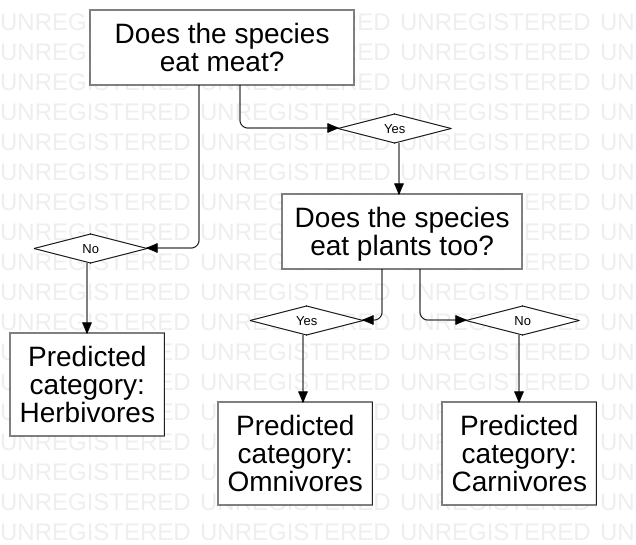
\includegraphics{/res/simple_decision_tree.png}
\caption{Simple Decision Tree (PNG)}
\end{figure}

    The process of recognizing patterns from data is called \textbf{fitting}
or \textbf{training}. The data used to \textbf{train} or \textbf{fit} is
called as \textbf{training data}.

There can be more complex, and thus more accurate decision trees. An
example of a more accurately predicting decision tree is given below:

\begin{figure}
\centering
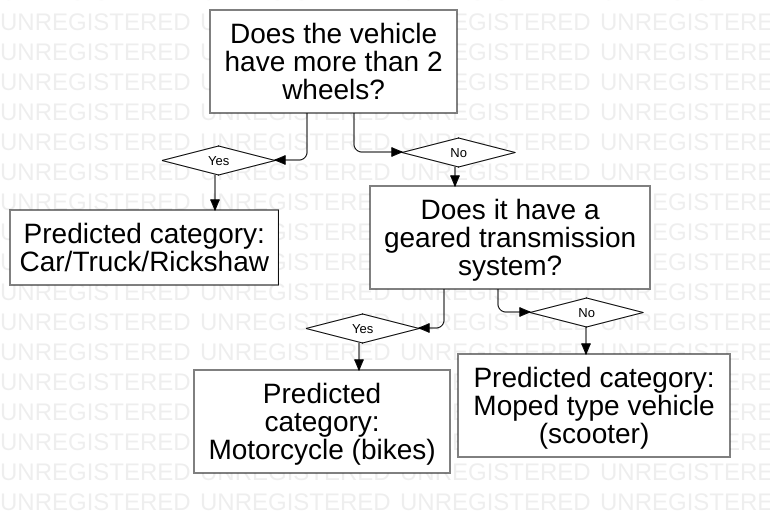
\includegraphics{/res/deeper_decision_tree.png}
\caption{Deeper Decision Tree (PNG)}
\end{figure}

This tree gives more accurate predictions than say a tree like the one
below:

\begin{figure}
\centering
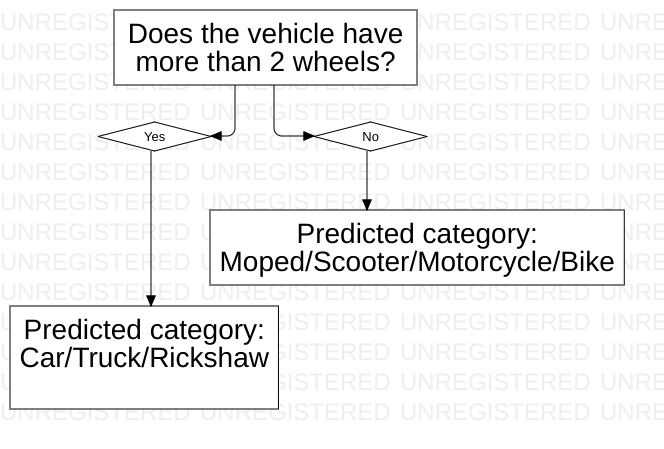
\includegraphics{/res/less_deep_decision_tree.png}
\caption{Less Deep Decision Tree (PNG)}
\end{figure}

    Deeper decision trees have more `\emph{splits}'. \emph{Splits} allow us
to introduce more number of \emph{factors} in our decision making
process. More the number of factors, better the prediction. The last
node of the tree, where we obtain our prediction, is known as the
\textbf{leaf} node.

    Let's use some data to try out our new tricks.

    \hypertarget{data-exploration-using-pandas}{%
\paragraph{Data exploration using
Pandas}\label{data-exploration-using-pandas}}

    Pandas is an open-source Python data analysis library. We can use Pandas
in our Python code by importing it. We generally import Pandas using the
abbreviation \textbf{pd}.

    \begin{Verbatim}[commandchars=\\\{\}]
{\color{incolor}In [{\color{incolor}2}]:} \PY{k+kn}{import} \PY{n+nn}{pandas} \PY{k}{as} \PY{n+nn}{pd}
\end{Verbatim}


    The most important feature of Pandas is its \textbf{\emph{DataFrame}}
object. A DataFrame is a container which holds the type of data which is
similar to a table or an Excel sheet or a SQL table. This DataFrame
object can then allow us to do a lot of things on the data using
powerful methods in the Pandas library.

As an example, we will be looking at data about home prices in
Melbourne, Australia.

    \begin{Verbatim}[commandchars=\\\{\}]
{\color{incolor}In [{\color{incolor}3}]:} \PY{c+c1}{\PYZsh{} saving filepath to a variable for easier access}
        \PY{n}{melb\PYZus{}data\PYZus{}filepath} \PY{o}{=} \PY{l+s+s1}{\PYZsq{}}\PY{l+s+s1}{res/melb\PYZus{}data.csv}\PY{l+s+s1}{\PYZsq{}}
        \PY{c+c1}{\PYZsh{} Read data from a CSV file and store it in a DataFrame object called melb\PYZus{}data}
        \PY{n}{melb\PYZus{}data} \PY{o}{=} \PY{n}{pd}\PY{o}{.}\PY{n}{read\PYZus{}csv}\PY{p}{(}\PY{n}{melb\PYZus{}data\PYZus{}filepath}\PY{p}{)}
        \PY{c+c1}{\PYZsh{} Print a summary of data in Melbourne data}
        \PY{n}{melb\PYZus{}data}\PY{o}{.}\PY{n}{describe}\PY{p}{(}\PY{p}{)}
\end{Verbatim}


\begin{Verbatim}[commandchars=\\\{\}]
{\color{outcolor}Out[{\color{outcolor}3}]:}               Rooms         Price      Distance      Postcode      Bedroom2  \textbackslash{}
        count  13580.000000  1.358000e+04  13580.000000  13580.000000  13580.000000   
        mean       2.937997  1.075684e+06     10.137776   3105.301915      2.914728   
        std        0.955748  6.393107e+05      5.868725     90.676964      0.965921   
        min        1.000000  8.500000e+04      0.000000   3000.000000      0.000000   
        25\%        2.000000  6.500000e+05      6.100000   3044.000000      2.000000   
        50\%        3.000000  9.030000e+05      9.200000   3084.000000      3.000000   
        75\%        3.000000  1.330000e+06     13.000000   3148.000000      3.000000   
        max       10.000000  9.000000e+06     48.100000   3977.000000     20.000000   
        
                   Bathroom           Car       Landsize  BuildingArea    YearBuilt  \textbackslash{}
        count  13580.000000  13518.000000   13580.000000   7130.000000  8205.000000   
        mean       1.534242      1.610075     558.416127    151.967650  1964.684217   
        std        0.691712      0.962634    3990.669241    541.014538    37.273762   
        min        0.000000      0.000000       0.000000      0.000000  1196.000000   
        25\%        1.000000      1.000000     177.000000     93.000000  1940.000000   
        50\%        1.000000      2.000000     440.000000    126.000000  1970.000000   
        75\%        2.000000      2.000000     651.000000    174.000000  1999.000000   
        max        8.000000     10.000000  433014.000000  44515.000000  2018.000000   
        
                  Lattitude    Longtitude  Propertycount  
        count  13580.000000  13580.000000   13580.000000  
        mean     -37.809203    144.995216    7454.417378  
        std        0.079260      0.103916    4378.581772  
        min      -38.182550    144.431810     249.000000  
        25\%      -37.856822    144.929600    4380.000000  
        50\%      -37.802355    145.000100    6555.000000  
        75\%      -37.756400    145.058305   10331.000000  
        max      -37.408530    145.526350   21650.000000  
\end{Verbatim}
            
    \hypertarget{interpreting-data-descriptions}{%
\paragraph{Interpreting data
descriptions}\label{interpreting-data-descriptions}}

    The table shows 8 numbers for all the columns in the original dataset.

The \textbf{count} column shows the number of rows containing
non-missing values. Missing values are those for which there is no
possible data. For example, the count for bedroom 2 in a 1 bedroom house
will not be available and thus missing.

The \textbf{mean} is an average of the values.

\textbf{std} is for the standard deviation of the values. Standard
deviation shows us how numerically the data is spread out. For more
about standard deviation, refer to the basic statistics section.

Sort the data in ascending order. The first value is the \textbf{min}
value. \textbf{25\%}, \textbf{50\%} and \textbf{75\%} are percentile
values (\emph{\(x^{th}\) percentile}). They indicate the values which
are bigger than \(x\)\% of the values in the dataset and smaller than
\((x - 100)\)\% of the values in the dataset. \textbf{max} is the
largest number.

    \hypertarget{selecting-data-for-modeling}{%
\paragraph{Selecting data for
modeling}\label{selecting-data-for-modeling}}

    The Melbourne housing problem dataset has a lot of variables in it. It
makes it difficult to grasp the data and understand it. We need to
narrow down the number of columns (or factors) to those which actually
matter. We will start by doing this intuitively.

The \textbf{columns} property of the DataFrame object allows us to see a
list of all the columns we have in our dataset.

    \begin{Verbatim}[commandchars=\\\{\}]
{\color{incolor}In [{\color{incolor}4}]:} \PY{c+c1}{\PYZsh{} We will continue our Python code from the last cell containing Python code}
        \PY{n}{melb\PYZus{}data}\PY{o}{.}\PY{n}{columns}
\end{Verbatim}


\begin{Verbatim}[commandchars=\\\{\}]
{\color{outcolor}Out[{\color{outcolor}4}]:} Index(['Suburb', 'Address', 'Rooms', 'Type', 'Price', 'Method', 'SellerG',
               'Date', 'Distance', 'Postcode', 'Bedroom2', 'Bathroom', 'Car',
               'Landsize', 'BuildingArea', 'YearBuilt', 'CouncilArea', 'Lattitude',
               'Longtitude', 'Regionname', 'Propertycount'],
              dtype='object')
\end{Verbatim}
            
    The Melbourne dataset contains rows with missing values. We will learn
how to handle missing values later, so for now we will just discard (or
drop) those rows. To do so, we will use the \textbf{dropna} method. The
\textbf{na} stands for \textbf{Not Available}.

    \begin{Verbatim}[commandchars=\\\{\}]
{\color{incolor}In [{\color{incolor}5}]:} \PY{n}{melb\PYZus{}data} \PY{o}{=} \PY{n}{melb\PYZus{}data}\PY{o}{.}\PY{n}{dropna}\PY{p}{(}\PY{n}{axis} \PY{o}{=} \PY{l+m+mi}{0}\PY{p}{)}
\end{Verbatim}


    \hypertarget{selecting-the-prediction-target}{%
\paragraph{Selecting the prediction
target}\label{selecting-the-prediction-target}}

Using Pandas, one can pull out a single variable using the
\emph{dot-notation}. This single column is stored in a
\textbf{\emph{Series}}. It is similar to a DataFrame but with only a
single column.

We will use the \emph{dot-notation} to select a column which is called a
\textbf{prediction target}. Our prediction target here would be the
house prices. By convention, the prediction target is stored in a
variable called \texttt{y}.

    \begin{Verbatim}[commandchars=\\\{\}]
{\color{incolor}In [{\color{incolor}6}]:} \PY{n}{y} \PY{o}{=} \PY{n}{melb\PYZus{}data}\PY{o}{.}\PY{n}{Price}
\end{Verbatim}


    \hypertarget{choosing-features}{%
\paragraph{Choosing features}\label{choosing-features}}

The columns in our dataset, which represent various variables, are known
as \emph{features}. Sometimes, we use all the columns (except our
target) in our dataset for prediction and sometimes, we need to filter
out some columns because they don't matter much or are not useful for
our prediction.

We can select multiple columns by providing our algorithm with an array
of all the columns which we want. Each column name should be of
\emph{string} datatype. For example:

    \begin{Verbatim}[commandchars=\\\{\}]
{\color{incolor}In [{\color{incolor}7}]:} \PY{n}{melb\PYZus{}features} \PY{o}{=} \PY{p}{[}\PY{l+s+s1}{\PYZsq{}}\PY{l+s+s1}{Rooms}\PY{l+s+s1}{\PYZsq{}}\PY{p}{,} \PY{l+s+s1}{\PYZsq{}}\PY{l+s+s1}{Bathroom}\PY{l+s+s1}{\PYZsq{}}\PY{p}{,} \PY{l+s+s1}{\PYZsq{}}\PY{l+s+s1}{Landsize}\PY{l+s+s1}{\PYZsq{}}\PY{p}{,} \PY{l+s+s1}{\PYZsq{}}\PY{l+s+s1}{Lattitude}\PY{l+s+s1}{\PYZsq{}}\PY{p}{,} \PY{l+s+s1}{\PYZsq{}}\PY{l+s+s1}{Longtitude}\PY{l+s+s1}{\PYZsq{}}\PY{p}{]}
\end{Verbatim}


    By convention, we denote this as \texttt{X}.

    \begin{Verbatim}[commandchars=\\\{\}]
{\color{incolor}In [{\color{incolor}8}]:} \PY{n}{X} \PY{o}{=} \PY{n}{melb\PYZus{}data}\PY{p}{[}\PY{n}{melb\PYZus{}features}\PY{p}{]}
\end{Verbatim}


    Let's have a look at the summary for \texttt{X}. After that, we shall
have a look at the first few rows of the data using the \textbf{head}
method.

    \begin{Verbatim}[commandchars=\\\{\}]
{\color{incolor}In [{\color{incolor}9}]:} \PY{n}{X}\PY{o}{.}\PY{n}{describe}\PY{p}{(}\PY{p}{)}
\end{Verbatim}


\begin{Verbatim}[commandchars=\\\{\}]
{\color{outcolor}Out[{\color{outcolor}9}]:}              Rooms     Bathroom      Landsize    Lattitude   Longtitude
        count  6196.000000  6196.000000   6196.000000  6196.000000  6196.000000
        mean      2.931407     1.576340    471.006940   -37.807904   144.990201
        std       0.971079     0.711362    897.449881     0.075850     0.099165
        min       1.000000     1.000000      0.000000   -38.164920   144.542370
        25\%       2.000000     1.000000    152.000000   -37.855438   144.926198
        50\%       3.000000     1.000000    373.000000   -37.802250   144.995800
        75\%       4.000000     2.000000    628.000000   -37.758200   145.052700
        max       8.000000     8.000000  37000.000000   -37.457090   145.526350
\end{Verbatim}
            
    \begin{Verbatim}[commandchars=\\\{\}]
{\color{incolor}In [{\color{incolor}10}]:} \PY{n}{X}\PY{o}{.}\PY{n}{head}\PY{p}{(}\PY{p}{)}
\end{Verbatim}


\begin{Verbatim}[commandchars=\\\{\}]
{\color{outcolor}Out[{\color{outcolor}10}]:}    Rooms  Bathroom  Landsize  Lattitude  Longtitude
         1      2       1.0     156.0   -37.8079    144.9934
         2      3       2.0     134.0   -37.8093    144.9944
         4      4       1.0     120.0   -37.8072    144.9941
         6      3       2.0     245.0   -37.8024    144.9993
         7      2       1.0     256.0   -37.8060    144.9954
\end{Verbatim}
            
    This check on data using visual methods is a very important job that
every data scientist should be skilled at. This is known as \textbf{data
visualization}.

    \hypertarget{building-the-model}{%
\paragraph{Building the model}\label{building-the-model}}

    We will use \textbf{scikit-learn} to build our model. It is a very
popular open-source library for building models using the type of data
which is stored using the DataFrame object. It is denoted by
\textbf{sklearn} in Python code.

The following are the steps followed while building and running a mdoel:

\begin{itemize}
\tightlist
\item
  \textbf{Define}: What type of a model will it be? Will it be a
  decision tree? Or something else? Other parameters related to the type
  of model are also specified at this step.
\item
  \textbf{Fit/Train}: Capture patterns in the provided data (training
  data). This is the most important step.
\item
  \textbf{Predict}: Self-explanatory.
\item
  \textbf{Evaluate}: Determine the accuracy of our model's predictions.
\end{itemize}

    Here is an example of a decision tree model using \textbf{scikit-learn}
and fitting it with features and target variable.

    \begin{Verbatim}[commandchars=\\\{\}]
{\color{incolor}In [{\color{incolor}11}]:} \PY{k+kn}{from} \PY{n+nn}{sklearn}\PY{n+nn}{.}\PY{n+nn}{tree} \PY{k}{import} \PY{n}{DecisionTreeRegressor}
         \PY{c+c1}{\PYZsh{} Define a model and set random\PYZus{}state to 1 to ensure same results after each run.}
         \PY{n}{melb\PYZus{}model} \PY{o}{=} \PY{n}{DecisionTreeRegressor}\PY{p}{(}\PY{n}{random\PYZus{}state}\PY{o}{=}\PY{l+m+mi}{1}\PY{p}{)}
         \PY{c+c1}{\PYZsh{} Fit the model.}
         \PY{n}{melb\PYZus{}model}\PY{o}{.}\PY{n}{fit}\PY{p}{(}\PY{n}{X}\PY{p}{,} \PY{n}{y}\PY{p}{)}
\end{Verbatim}


\begin{Verbatim}[commandchars=\\\{\}]
{\color{outcolor}Out[{\color{outcolor}11}]:} DecisionTreeRegressor(criterion='mse', max\_depth=None, max\_features=None,
                    max\_leaf\_nodes=None, min\_impurity\_decrease=0.0,
                    min\_impurity\_split=None, min\_samples\_leaf=1,
                    min\_samples\_split=2, min\_weight\_fraction\_leaf=0.0,
                    presort=False, random\_state=1, splitter='best')
\end{Verbatim}
            
    Many machine learning models allow some randomness in their model
training. When we specify a number for \texttt{random\_state}, we are
ensuring that we get the same result in each run. This is considered as
good practice. The model quality won't depend on the value of
\texttt{random\_state} that you choose.

We now have fitted a model which we can use to predict value. In
practice, we will make predictions for the newer houses being built,
but, for now, we will make predictions for the first few rows of the
dataset just to see how our model performs.

    \begin{Verbatim}[commandchars=\\\{\}]
{\color{incolor}In [{\color{incolor}12}]:} \PY{n+nb}{print}\PY{p}{(}\PY{l+s+s2}{\PYZdq{}}\PY{l+s+s2}{Making predictions for the following 5 houses:}\PY{l+s+s2}{\PYZdq{}}\PY{p}{)}\PY{p}{;}
         \PY{n+nb}{print}\PY{p}{(}\PY{n}{X}\PY{o}{.}\PY{n}{head}\PY{p}{(}\PY{p}{)}\PY{p}{)}
         \PY{n+nb}{print}\PY{p}{(}\PY{l+s+s2}{\PYZdq{}}\PY{l+s+s2}{The predictions are:}\PY{l+s+s2}{\PYZdq{}}\PY{p}{)}
         \PY{n+nb}{print}\PY{p}{(}\PY{n}{melb\PYZus{}model}\PY{o}{.}\PY{n}{predict}\PY{p}{(}\PY{n}{X}\PY{o}{.}\PY{n}{head}\PY{p}{(}\PY{p}{)}\PY{p}{)}\PY{p}{)}
\end{Verbatim}


    \begin{Verbatim}[commandchars=\\\{\}]
Making predictions for the following 5 houses:
   Rooms  Bathroom  Landsize  Lattitude  Longtitude
1      2       1.0     156.0   -37.8079    144.9934
2      3       2.0     134.0   -37.8093    144.9944
4      4       1.0     120.0   -37.8072    144.9941
6      3       2.0     245.0   -37.8024    144.9993
7      2       1.0     256.0   -37.8060    144.9954
The predictions are:
[1035000. 1465000. 1600000. 1876000. 1636000.]

    \end{Verbatim}

    Now that we have built a decision tree model, it is natural to ask how
accurate our model's predictions are and how to improve them. We can do
that with model validation.

    \hypertarget{model-validation}{%
\paragraph{Model Validation}\label{model-validation}}

    Model validation is used to measure the \textbf{quality of the model}.
The quality of the model is the key to iteratively improve upon the
model. We will likely want to assess the quality of every model we ever
build, and in most cases, the \emph{predictive accuracy} is a very
relevant measure of model quality. In easier words, we want to know how
close the predictions given by a model are to what actually happens.

A lot of people make a big mistake when validating a model. They use the
\emph{training} data to make predictions and compare the predicted
results with the target variable in the \emph{training} data. We shall
see the problems which occur when using the \emph{training} data for
predictions later on. One should insteead use the \emph{testing} data
for making the predictions.

Our data may have tens of thousands of rows of data. To compare the
predicted and actual values to asses the model quality by labelling each
row's prediction to be either good or bad would take a lot of manpower
and time. Instead, we need to summarize the whole set of data and the
predictions into one single metric. There are many metrics for
summarizing the model quality, but we shall have a look at a basic one
called \textbf{Mean Absolute Error (MAE)}.

The prediction error for each row (each house here) of data would be

\begin{verbatim}
error = actual - predicted
\end{verbatim}

    Thus, if a house costs \textbackslash{}\$100,000 and the predicted price
was \textbackslash{}\$80,000, then the error is
\textbackslash{}\$20,000.

    We take the absolute value of errors in the \textbf{MAE} metric. Then we
take the average of these absolute errors. This average is our
\textbf{MAE} for that data. In short, \textbf{Mean Absolute Error}
means, ``on average, our predictions are off by about X''.

    Let's find the MAE for our Melbourne model (\texttt{melb\_model}).

    \begin{Verbatim}[commandchars=\\\{\}]
{\color{incolor}In [{\color{incolor}13}]:} \PY{k+kn}{from} \PY{n+nn}{sklearn}\PY{n+nn}{.}\PY{n+nn}{metrics} \PY{k}{import} \PY{n}{mean\PYZus{}absolute\PYZus{}error}
         \PY{n}{predicted\PYZus{}home\PYZus{}prices} \PY{o}{=} \PY{n}{melb\PYZus{}model}\PY{o}{.}\PY{n}{predict}\PY{p}{(}\PY{n}{X}\PY{p}{)}
         \PY{n}{mean\PYZus{}absolute\PYZus{}error}\PY{p}{(}\PY{n}{y}\PY{p}{,} \PY{n}{predicted\PYZus{}home\PYZus{}prices}\PY{p}{)}
\end{Verbatim}


\begin{Verbatim}[commandchars=\\\{\}]
{\color{outcolor}Out[{\color{outcolor}13}]:} 1115.7467183128902
\end{Verbatim}
            
    What we obtained is known as an ``\textbf{In-sample}'' score. An
in-sample score is the one which is obtained where the data or the
``\textbf{sample}'' used for predictions is the same as the one used to
train or build the model.

What our model does is recognize patterns in the data. Now, when we
predict the model using the same data, it will definitely recognize the
patterns and will predict accurately. But what if we introduce some data
to predict which is not present in the original dataset (or the dataset
used to train the model)? The model should still predict with the same
accuracy. If it doesn't, it indicates a low quality of our model.

In real life, we don't make predictions for the data for which we
already have the answers, but we use unknown data which the model might
not have ever seen before and we predict results for that data. If the
results for unknown data are accurate, it indicates a high quality of
our model. Our model is performing well then.

We exclude some data from our original dataset while building our model
and use that excluded data which the model has never seen before to test
our model's performance. This excluded data is known as
\textbf{validation data} or \textbf{testing data}. The data used for
building or training the model is known as \textbf{training data}.

\textbf{scikit-learn} provides us with a method to split the data into
\emph{training} and \emph{testing}. It is called
\texttt{train\_test\_split}.

    Let's try out the Melbourne Housing Prices problem after splitting our
data into \textbf{training data} and \textbf{validation data}.

The split done using \texttt{train\_test\_split} is based on a random
number generator. Using a \texttt{random\_state} value with
\texttt{train\_test\_split} ensures that we get the same split every
time we run the code.

    \begin{Verbatim}[commandchars=\\\{\}]
{\color{incolor}In [{\color{incolor}14}]:} \PY{k+kn}{from} \PY{n+nn}{sklearn}\PY{n+nn}{.}\PY{n+nn}{model\PYZus{}selection} \PY{k}{import} \PY{n}{train\PYZus{}test\PYZus{}split}
         \PY{n}{train\PYZus{}X}\PY{p}{,} \PY{n}{val\PYZus{}X}\PY{p}{,} \PY{n}{train\PYZus{}y}\PY{p}{,} \PY{n}{val\PYZus{}y} \PY{o}{=} \PY{n}{train\PYZus{}test\PYZus{}split}\PY{p}{(}\PY{n}{X}\PY{p}{,} \PY{n}{y}\PY{p}{,} \PY{n}{random\PYZus{}state} \PY{o}{=} \PY{l+m+mi}{0}\PY{p}{)}
         \PY{n}{melb\PYZus{}model} \PY{o}{=} \PY{n}{DecisionTreeRegressor}\PY{p}{(}\PY{p}{)}
         \PY{n}{melb\PYZus{}model}\PY{o}{.}\PY{n}{fit}\PY{p}{(}\PY{n}{train\PYZus{}X}\PY{p}{,} \PY{n}{train\PYZus{}y}\PY{p}{)}
         \PY{n}{val\PYZus{}predictions} \PY{o}{=} \PY{n}{melb\PYZus{}model}\PY{o}{.}\PY{n}{predict}\PY{p}{(}\PY{n}{val\PYZus{}X}\PY{p}{)}
         \PY{n+nb}{print}\PY{p}{(}\PY{n}{mean\PYZus{}absolute\PYZus{}error}\PY{p}{(}\PY{n}{val\PYZus{}y}\PY{p}{,} \PY{n}{val\PYZus{}predictions}\PY{p}{)}\PY{p}{)}
\end{Verbatim}


    \begin{Verbatim}[commandchars=\\\{\}]
273133.84828921885

    \end{Verbatim}

    Thus, when the model was trained and tested using the same data, it
reported am error of \textbackslash{}\$1116 and when it was trained and
tested using different data, it reported a massive error of about
\textbackslash{}\$271,900.

This proves that our model is \textbf{not a valid one}. It does not
predict housing prices very accurately.

    \hypertarget{underfitting-and-overfitting}{%
\paragraph{Underfitting and
Overfitting}\label{underfitting-and-overfitting}}

    So, now that we have learnt how to measure the quality of a model and
how to determine its validity, we can experiment with alternate models
and find out which one is the better one for our application. But what
alternatives can we have for our model?

The documentation for \texttt{scikit-learn} library's \emph{decision
tree} model reveals the many different options we can use along with it.
One of the most important ones are for finding the depth of the decision
tree. We have used very shallow ones till now.

It is not very uncommon for decision trees to have 10 splits, or a depth
of 10, in real world applications of machine learning. This will create
a lot of leaf nodes. For 1 split, we divide our dataset into \(2\)
groups. A further 2nd split will divide it into \(4\) groups. Further,
if all the leaf nodes are split, it will divide it into \(8\) groups and
so on. If we have a decision tree with 10 splits, it will have
\(2^{10}\) leaf nodes, which is equal to 1024 leaf nodes. Thus, the
number of leaf nodes in a decision tree grows exponentially and can be
found as follows:

\[
leaf nodes = 2^{d}
\]

where, \(d\) is the depth of the decision tree (or the number of splits
a decision tree has).

As we split the leaf nodes, the number of houses in them decreases. At
first, we had the whole dataset. Then, after the first split, the
dataset was divided into \(2\) groups. Each of these groups have the
number of houses less than what was there before the split. A fursther
split will divide each of these groups into more smaller sets.

Leaves with very few houses in them will make predictions that are quite
close to those homes' actual values, but they make very unreliable
predictions for new data, because each of these predictions is based
only on few houses.

This phenomenon is called \textbf{overfitting}, where the model matches
the training data perfectly but doesn't hold good for newer data and
validation.

On the flip side, a shallow tree gives us very few groups to divide our
data into, distinctively. In some cases, when a tree has only 2 or 4
splits, the number of groups is less and each of these groups will
contain data that is diverse and of different categories. The
predictions for most of the houses will be far from the actual value.

The training dataset will not match with the model and even the
validation data won't be matched properly. When a model fails to capture
important distinctions and patterns in the data and thus performs poorly
on both, the training data and the validation data, it is called
\textbf{underfitting}.

Thus, our goal is to find the sweet spot between overfitting and
underfitting.

As the depth of the tree increases, the MAE decreases. Thus, for
underfitting, the MAE is high for both, training data and validation
data. For overfitting, the value of MAE is high for validation data.

Thus, for training data, when the depth of the tree is small
(underfitting), the MAE is high. As we increase the depth, MAE
decreases. For validation data, when the depth of the tree is small, the
value of MAE is high (underfitting). As we increase the depth of the
tree, MAE decreases (sweet spot), and when we increase the depth of the
tree still more, MAE for validation data starts increasing
(overfitting).

    There are a few methods to control the depth of a decision tree, and
some even allow a decision tree to have variable length for different
routes. \texttt{scikit-learn} provides us with the
\texttt{max\_leaf\_nodes} argument which allows us to set a value for
the maximum number of leaf nodes a decision tree can have. This allows
us with a very basic, but sensible way to control overfitting and
underfitting.

The more the leaves we allow, the further we move away from underfitting
towards overfitting.

We can compare the MAE values for different values of
\texttt{max\_leaf\_nodes} using a utility function as demonstrated
below.

    \begin{Verbatim}[commandchars=\\\{\}]
{\color{incolor}In [{\color{incolor}15}]:} \PY{k+kn}{from} \PY{n+nn}{sklearn}\PY{n+nn}{.}\PY{n+nn}{metrics} \PY{k}{import} \PY{n}{mean\PYZus{}absolute\PYZus{}error}
         \PY{k+kn}{from} \PY{n+nn}{sklearn}\PY{n+nn}{.}\PY{n+nn}{tree} \PY{k}{import} \PY{n}{DecisionTreeRegressor}
         
         \PY{k}{def} \PY{n+nf}{get\PYZus{}mae}\PY{p}{(}\PY{n}{max\PYZus{}leaf\PYZus{}nodes}\PY{p}{,} \PY{n}{train\PYZus{}X}\PY{p}{,} \PY{n}{val\PYZus{}X}\PY{p}{,} \PY{n}{train\PYZus{}y}\PY{p}{,} \PY{n}{val\PYZus{}y}\PY{p}{)}\PY{p}{:}
             \PY{n}{model} \PY{o}{=} \PY{n}{DecisionTreeRegressor}\PY{p}{(}\PY{n}{max\PYZus{}leaf\PYZus{}nodes} \PY{o}{=} \PY{n}{max\PYZus{}leaf\PYZus{}nodes}\PY{p}{,} \PY{n}{random\PYZus{}state} \PY{o}{=} \PY{l+m+mi}{0}\PY{p}{)}
             \PY{n}{model}\PY{o}{.}\PY{n}{fit}\PY{p}{(}\PY{n}{train\PYZus{}X}\PY{p}{,} \PY{n}{train\PYZus{}y}\PY{p}{)}
             \PY{n}{preds\PYZus{}val} \PY{o}{=} \PY{n}{model}\PY{o}{.}\PY{n}{predict}\PY{p}{(}\PY{n}{val\PYZus{}X}\PY{p}{)}
             \PY{n}{mae} \PY{o}{=} \PY{n}{mean\PYZus{}absolute\PYZus{}error}\PY{p}{(}\PY{n}{val\PYZus{}y}\PY{p}{,} \PY{n}{preds\PYZus{}val}\PY{p}{)}
             \PY{k}{return}\PY{p}{(}\PY{n}{mae}\PY{p}{)}
\end{Verbatim}


    We can use a for-loop to compare the accuracy of models built with
different values for \texttt{max\_leaf\_nodes}.

    \begin{Verbatim}[commandchars=\\\{\}]
{\color{incolor}In [{\color{incolor}16}]:} \PY{c+c1}{\PYZsh{} compare MAE with differing values of max\PYZus{}leaf\PYZus{}nodes}
         \PY{k}{for} \PY{n}{max\PYZus{}leaf\PYZus{}nodes} \PY{o+ow}{in} \PY{p}{[}\PY{l+m+mi}{5}\PY{p}{,} \PY{l+m+mi}{50}\PY{p}{,} \PY{l+m+mi}{500}\PY{p}{,} \PY{l+m+mi}{5000}\PY{p}{]}\PY{p}{:}
             \PY{n}{my\PYZus{}mae} \PY{o}{=} \PY{n}{get\PYZus{}mae}\PY{p}{(}\PY{n}{max\PYZus{}leaf\PYZus{}nodes}\PY{p}{,} \PY{n}{train\PYZus{}X}\PY{p}{,} \PY{n}{val\PYZus{}X}\PY{p}{,} \PY{n}{train\PYZus{}y}\PY{p}{,} \PY{n}{val\PYZus{}y}\PY{p}{)}
             \PY{n+nb}{print}\PY{p}{(}\PY{l+s+s2}{\PYZdq{}}\PY{l+s+s2}{Max leaf nodes: }\PY{l+s+si}{\PYZpc{}d}\PY{l+s+se}{\PYZbs{}t}\PY{l+s+se}{\PYZbs{}t}\PY{l+s+s2}{Mean Absolute Error: }\PY{l+s+si}{\PYZpc{}d}\PY{l+s+s2}{\PYZdq{}} \PY{o}{\PYZpc{}}\PY{p}{(}\PY{n}{max\PYZus{}leaf\PYZus{}nodes}\PY{p}{,} \PY{n}{my\PYZus{}mae}\PY{p}{)}\PY{p}{)}
\end{Verbatim}


    \begin{Verbatim}[commandchars=\\\{\}]
Max leaf nodes: 5		Mean Absolute Error: 385696
Max leaf nodes: 50		Mean Absolute Error: 279794
Max leaf nodes: 500		Mean Absolute Error: 261718
Max leaf nodes: 5000		Mean Absolute Error: 271996

    \end{Verbatim}

    Here, we can see that 500 is the optimal number of leaf nodes that we
should have for our model.

    \hypertarget{random-forests}{%
\paragraph{Random Forests}\label{random-forests}}

Decision trees make us take a very difficult decision. Should we create
a deep tree with lots of leaf nodes which will overfit because each
prediction is coming from historical data of only a few houses present
at the leaf \emph{or} should we create a shallow decision tree with a
less number of leaf nodes which will perform poorly because it fails to
capture as many distinctions in the raw data?

Many modern and complex models face this problem of finding that
harmoniuos balance between underfitting and overfitting. Some models
have very clever ideas to overcome this problem which leads to better
performance. One of them is known as \textbf{Random Forests}.

    Random forests use multiple decision trees. It makes predictions by
averaging the predictions of each component trees. It generally has
better prediction accuracy as compared to a single decision tree. It
works well with the default parameters. Many other models have even
better performance than random forests, but they are sensitive to
getting the right parameters.

    We already know how to load our data. We split our data into two sets:
one for training and the other for validation. We do so using the
following varibales:

\begin{itemize}
\tightlist
\item
  train\_X
\item
  val\_X
\item
  train\_y
\item
  val\_y
\end{itemize}

Building a random forest is similar to what we did while building a
decision tree in terms of Python code. We use \texttt{scikit-learn} and
import the \texttt{RandomForestRegressor} instead of
\texttt{DecisionTreeRegressor}.

    \begin{Verbatim}[commandchars=\\\{\}]
{\color{incolor}In [{\color{incolor}20}]:} \PY{k+kn}{from} \PY{n+nn}{sklearn}\PY{n+nn}{.}\PY{n+nn}{ensemble} \PY{k}{import} \PY{n}{RandomForestRegressor}
         \PY{k+kn}{from} \PY{n+nn}{sklearn}\PY{n+nn}{.}\PY{n+nn}{metrics} \PY{k}{import} \PY{n}{mean\PYZus{}absolute\PYZus{}error}
         
         \PY{n}{forest\PYZus{}model} \PY{o}{=} \PY{n}{RandomForestRegressor}\PY{p}{(}\PY{n}{random\PYZus{}state} \PY{o}{=} \PY{l+m+mi}{1}\PY{p}{)}
         \PY{n}{forest\PYZus{}model}\PY{o}{.}\PY{n}{fit}\PY{p}{(}\PY{n}{train\PYZus{}X}\PY{p}{,} \PY{n}{train\PYZus{}y}\PY{p}{)}
         \PY{n}{melb\PYZus{}preds} \PY{o}{=} \PY{n}{forest\PYZus{}model}\PY{o}{.}\PY{n}{predict}\PY{p}{(}\PY{n}{val\PYZus{}X}\PY{p}{)}
         \PY{n+nb}{print}\PY{p}{(}\PY{n}{mean\PYZus{}absolute\PYZus{}error}\PY{p}{(}\PY{n}{val\PYZus{}y}\PY{p}{,} \PY{n}{melb\PYZus{}preds}\PY{p}{)}\PY{p}{)}
\end{Verbatim}


    \begin{Verbatim}[commandchars=\\\{\}]
218482.25517538196

    \end{Verbatim}

    \begin{Verbatim}[commandchars=\\\{\}]
/home/hpd/miniconda3/envs/AI/lib/python3.7/site-packages/sklearn/ensemble/forest.py:246: FutureWarning: The default value of n\_estimators will change from 10 in version 0.20 to 100 in 0.22.
  "10 in version 0.20 to 100 in 0.22.", FutureWarning)

    \end{Verbatim}

    There is always room for more improvement, but this is a very good
improvement in itself as compared to the MAE we got using a single
decision tree.

We can set parameters which allow us to further tune and improve upon
the performance of the random forest as we did by setting the maximum
depth of a tree while using a single decision tree. But, the best
feature of a random forest is that it works well even without setting
the parameters and tuning it. We will soon learn the XGBoost model which
will vastly improve the performance when tuned with the right set of
parameters. This requires a bit of more skills to get the right
parameters set.

    \hypertarget{numpy}{%
\subsubsection{NumPy}\label{numpy}}

\hypertarget{basics}{%
\paragraph{Basics}\label{basics}}

NumPy is a Python library which provides us with support for large
multi-dimensional arrays and matrices. It also provides high-level
mathematical functions to operate on these arrays.

NumPy's main object is a \emph{homogeneous multi-dimensional} array. It
is a table of elements which are mostly numeric. All elements in an
array are of the same type. They are indexed by a tuple of positive
integers.

In NumPy, \emph{dimensions} are called \textbf{axes}.

    Example,

\begin{verbatim}
[1, 3, 8]
\end{verbatim}

The above given array has 1 axis and that axis contains 2 elements.
Thus, the length of that axis is 2.

\begin{verbatim}
[[3, 1, 6],
[5, 5, 0]]
\end{verbatim}

The above given array has 2 axes. The first axis contains 2 elements
(\texttt{{[}3,\ 1,\ 6{]}} and \texttt{{[}5,\ 5,\ 0{]}}). The second axis
contains 3 elements (\texttt{3}, \texttt{1} and \texttt{6})(\texttt{5},
\texttt{5} and \texttt{0}).

    NumPy's array class is known as \texttt{ndarray} which stands for
\textbf{n-dimensional array}. \texttt{ndarray} is aliased by
\texttt{array}. The standard Python array class, \texttt{array.array} is
not the same as NumPy's array class, \texttt{numpy.array}.
\texttt{array.array} offer way less functionality and handles only
1-dimensional arrays.

Following are the important attributes of the \texttt{ndarray} class:

\begin{itemize}
\item
  \textbf{\texttt{ndarray.ndim}}

  The number of axes (dimensions) of the array.
\item
  \textbf{\texttt{ndarray.shape}}

  This is a tuple of integers which indicate the size of the array in
  each dimension. For example, for a matrix with \emph{n} rows and
  \emph{m} columns, the \texttt{shape} would be \texttt{(n,\ m)}. The
  length of the \texttt{shape} tuple is therefore the number of axes,
  \texttt{ndim}.
\item
  \textbf{\texttt{ndarray.size}}

  This gives us the total number of elements of an array. It is equal to
  the product of the elements of \texttt{shape}.
\item
  \textbf{\texttt{ndarray.dtype}}

  This is an object describing the type of the elements in the array.
  \texttt{dtype}s can be specified using standard Python types.
  Additionally, NumPy provides with its own types like
  \texttt{numpy.int32}, \texttt{numpy.int16}, \texttt{numpy.float64}.
\item
  \textbf{\texttt{ndarray.itemsize}}

  This gives us the size in bytes of each element of the array. For
  example, for an array of elements of type \texttt{float64}, the size
  would be 8 (8 bytes = 64 bits), for an array of elements of type
  \texttt{complex32}, the size would be 4 (4 bytes = 32 bits).
  \texttt{ndarray.itemsize} is equivalent to
  \texttt{ndarray.dtype.itemsize}.
\item
  \textbf{\texttt{ndarray.data}}

  This is the buffer containing the actual elements of an array.
  Normally, we won't require this as we will access elements using
  indexing facilities.
\end{itemize}

    Let's check out how to use NumPy in our code. We use NumPy in our Python
code as \texttt{np}.

    \begin{Verbatim}[commandchars=\\\{\}]
{\color{incolor}In [{\color{incolor} }]:} \PY{k+kn}{import} \PY{n+nn}{numpy} \PY{k}{as} \PY{n+nn}{np}
\end{Verbatim}


    Let's try out the above given attributes with examples.

    \begin{Verbatim}[commandchars=\\\{\}]
{\color{incolor}In [{\color{incolor} }]:} \PY{n}{array0} \PY{o}{=} \PY{n}{np}\PY{o}{.}\PY{n}{arange}\PY{p}{(}\PY{l+m+mi}{15}\PY{p}{)}
        \PY{n}{array0}
\end{Verbatim}


    The \texttt{arange} method allows us to create an array with integer
elements from \texttt{0} to the value passed to the \texttt{arange}
method.

    \begin{Verbatim}[commandchars=\\\{\}]
{\color{incolor}In [{\color{incolor} }]:} \PY{n}{array0} \PY{o}{=} \PY{n}{array0}\PY{o}{.}\PY{n}{reshape}\PY{p}{(}\PY{l+m+mi}{3}\PY{p}{,} \PY{l+m+mi}{5}\PY{p}{)}
        \PY{n}{array0}
\end{Verbatim}


    The \texttt{reshape} method allows us to change the shape of our array.
The \texttt{3,\ 5} mean that the array will display as a matrix of 3
rows with 5 columns.

    \begin{Verbatim}[commandchars=\\\{\}]
{\color{incolor}In [{\color{incolor} }]:} \PY{n}{array0}\PY{o}{.}\PY{n}{shape}
\end{Verbatim}


    \begin{Verbatim}[commandchars=\\\{\}]
{\color{incolor}In [{\color{incolor} }]:} \PY{n}{array1} \PY{o}{=} \PY{n}{np}\PY{o}{.}\PY{n}{arange}\PY{p}{(}\PY{l+m+mi}{18}\PY{p}{)}\PY{o}{.}\PY{n}{reshape}\PY{p}{(}\PY{l+m+mi}{6}\PY{p}{,} \PY{l+m+mi}{3}\PY{p}{)}
        \PY{n}{array1}
\end{Verbatim}


    \begin{Verbatim}[commandchars=\\\{\}]
{\color{incolor}In [{\color{incolor} }]:} \PY{n}{array1}\PY{o}{.}\PY{n}{shape}
\end{Verbatim}


    \begin{Verbatim}[commandchars=\\\{\}]
{\color{incolor}In [{\color{incolor} }]:} \PY{n}{array0}\PY{o}{.}\PY{n}{ndim}
\end{Verbatim}


    \begin{Verbatim}[commandchars=\\\{\}]
{\color{incolor}In [{\color{incolor} }]:} \PY{n}{array2} \PY{o}{=} \PY{n}{np}\PY{o}{.}\PY{n}{array}\PY{p}{(}\PY{p}{[}\PY{p}{[}\PY{p}{[}\PY{l+m+mi}{1}\PY{p}{,} \PY{l+m+mi}{2}\PY{p}{]}\PY{p}{,} \PY{p}{[}\PY{l+m+mi}{2}\PY{p}{,} \PY{l+m+mi}{3}\PY{p}{]}\PY{p}{]}\PY{p}{,} \PY{p}{[}\PY{p}{[}\PY{l+m+mi}{3}\PY{p}{,} \PY{l+m+mi}{4}\PY{p}{]}\PY{p}{,} \PY{p}{[}\PY{l+m+mi}{4}\PY{p}{,} \PY{l+m+mi}{5}\PY{p}{]}\PY{p}{]}\PY{p}{]}\PY{p}{)}
        \PY{n}{array2}
\end{Verbatim}


    \begin{Verbatim}[commandchars=\\\{\}]
{\color{incolor}In [{\color{incolor} }]:} \PY{n}{array2}\PY{o}{.}\PY{n}{ndim}
\end{Verbatim}


    \begin{Verbatim}[commandchars=\\\{\}]
{\color{incolor}In [{\color{incolor} }]:} \PY{n}{array0}\PY{o}{.}\PY{n}{dtype}
\end{Verbatim}


    \begin{Verbatim}[commandchars=\\\{\}]
{\color{incolor}In [{\color{incolor} }]:} \PY{n}{array0\PYZus{}dtype} \PY{o}{=} \PY{n}{array0}\PY{o}{.}\PY{n}{dtype}\PY{o}{.}\PY{n}{name}
        \PY{n}{array1\PYZus{}dtype} \PY{o}{=} \PY{n}{array1}\PY{o}{.}\PY{n}{dtype}\PY{o}{.}\PY{n}{name}
        \PY{n}{array2\PYZus{}dtype} \PY{o}{=} \PY{n}{array2}\PY{o}{.}\PY{n}{dtype}\PY{o}{.}\PY{n}{name}
        \PY{n+nb}{print}\PY{p}{(}\PY{n}{array0\PYZus{}dtype}\PY{p}{)}
        \PY{n+nb}{print}\PY{p}{(}\PY{n}{array1\PYZus{}dtype}\PY{p}{)}
        \PY{n+nb}{print}\PY{p}{(}\PY{n}{array2\PYZus{}dtype}\PY{p}{)}
\end{Verbatim}


    The \texttt{name} feature of any \texttt{dtype} object extracts the name
of the type of data.

    \begin{Verbatim}[commandchars=\\\{\}]
{\color{incolor}In [{\color{incolor} }]:} \PY{n}{itemsize\PYZus{}array0} \PY{o}{=} \PY{n}{array0}\PY{o}{.}\PY{n}{itemsize}
        \PY{n}{itemsize\PYZus{}array1} \PY{o}{=} \PY{n}{array1}\PY{o}{.}\PY{n}{itemsize}
        \PY{n}{itemsize\PYZus{}array2} \PY{o}{=} \PY{n}{array2}\PY{o}{.}\PY{n}{itemsize}
        \PY{n+nb}{print}\PY{p}{(}\PY{n}{itemsize\PYZus{}array0}\PY{p}{)}
        \PY{n+nb}{print}\PY{p}{(}\PY{n}{itemsize\PYZus{}array1}\PY{p}{)}
        \PY{n+nb}{print}\PY{p}{(}\PY{n}{itemsize\PYZus{}array2}\PY{p}{)}
\end{Verbatim}


    \begin{Verbatim}[commandchars=\\\{\}]
{\color{incolor}In [{\color{incolor} }]:} \PY{n}{size\PYZus{}array0} \PY{o}{=} \PY{n}{array0}\PY{o}{.}\PY{n}{size}
        \PY{n}{size\PYZus{}array1} \PY{o}{=} \PY{n}{array1}\PY{o}{.}\PY{n}{size}
        \PY{n}{size\PYZus{}array2} \PY{o}{=} \PY{n}{array2}\PY{o}{.}\PY{n}{size}
        \PY{n+nb}{print}\PY{p}{(}\PY{n}{size\PYZus{}array0}\PY{p}{)}
        \PY{n+nb}{print}\PY{p}{(}\PY{n}{size\PYZus{}array1}\PY{p}{)}
        \PY{n+nb}{print}\PY{p}{(}\PY{n}{size\PYZus{}array2}\PY{p}{)}
\end{Verbatim}


    \begin{Verbatim}[commandchars=\\\{\}]
{\color{incolor}In [{\color{incolor} }]:} \PY{n+nb}{type}\PY{p}{(}\PY{n}{array0}\PY{p}{)}
\end{Verbatim}


    \begin{Verbatim}[commandchars=\\\{\}]
{\color{incolor}In [{\color{incolor} }]:} \PY{n+nb}{type}\PY{p}{(}\PY{n}{array2}\PY{p}{)}
\end{Verbatim}


    \hypertarget{array-creation}{%
\paragraph{Array creation}\label{array-creation}}

There are several ways of creating arrays using NumPy.

One can create arrays using a regular Python list or tuple using the
\texttt{array} function. The type of the array obtained is automatically
determined from the type of elements in the sequences.

    \begin{Verbatim}[commandchars=\\\{\}]
{\color{incolor}In [{\color{incolor} }]:} \PY{k+kn}{import} \PY{n+nn}{numpy} \PY{k}{as} \PY{n+nn}{np}
        \PY{n}{array3} \PY{o}{=} \PY{n}{np}\PY{o}{.}\PY{n}{array}\PY{p}{(}\PY{p}{[}\PY{l+m+mi}{1}\PY{p}{,} \PY{l+m+mi}{2}\PY{p}{,} \PY{l+m+mi}{3}\PY{p}{,} \PY{l+m+mi}{4}\PY{p}{,} \PY{l+m+mi}{5}\PY{p}{]}\PY{p}{)}
        \PY{n}{array3}
\end{Verbatim}


    \begin{Verbatim}[commandchars=\\\{\}]
{\color{incolor}In [{\color{incolor} }]:} \PY{n}{array3}\PY{o}{.}\PY{n}{dtype}
\end{Verbatim}


    \begin{Verbatim}[commandchars=\\\{\}]
{\color{incolor}In [{\color{incolor} }]:} \PY{n}{array4} \PY{o}{=} \PY{n}{np}\PY{o}{.}\PY{n}{array}\PY{p}{(}\PY{p}{[}\PY{l+m+mf}{3.2}\PY{p}{,} \PY{l+m+mf}{5.1}\PY{p}{,} \PY{l+m+mf}{4.4}\PY{p}{,} \PY{l+m+mf}{8.2}\PY{p}{]}\PY{p}{)}
        \PY{n}{array4}
\end{Verbatim}


    \begin{Verbatim}[commandchars=\\\{\}]
{\color{incolor}In [{\color{incolor} }]:} \PY{n}{array4}\PY{o}{.}\PY{n}{dtype}
\end{Verbatim}


    Many times, a very common mistake which we tend to make is calling
\texttt{array} with \textbf{multiple numeric} arguments instead of
providing a \textbf{single list of numbers} as an argument.

    \begin{Verbatim}[commandchars=\\\{\}]
{\color{incolor}In [{\color{incolor} }]:} \PY{n}{array5} \PY{o}{=} \PY{n}{np}\PY{o}{.}\PY{n}{array}\PY{p}{(}\PY{l+m+mi}{1}\PY{p}{,} \PY{l+m+mi}{2}\PY{p}{,} \PY{l+m+mi}{3}\PY{p}{,} \PY{l+m+mi}{4}\PY{p}{)}
\end{Verbatim}


    This is \textbf{WRONG} and will show an error as above.

    The proper way to do that would be as follows:

    \begin{Verbatim}[commandchars=\\\{\}]
{\color{incolor}In [{\color{incolor} }]:} \PY{n}{array6} \PY{o}{=} \PY{n}{np}\PY{o}{.}\PY{n}{array}\PY{p}{(}\PY{p}{[}\PY{l+m+mi}{1}\PY{p}{,} \PY{l+m+mi}{2}\PY{p}{,} \PY{l+m+mi}{3}\PY{p}{,} \PY{l+m+mi}{4}\PY{p}{]}\PY{p}{)}
\end{Verbatim}


    \texttt{array} transforms \textbf{\emph{sequences of sequences}} into
\textbf{\emph{two-dimensional}} arrays, \textbf{\emph{sequences of
sequences of sequences}} into \textbf{\emph{three-dimensional}} arrays,
and so on.

    \begin{Verbatim}[commandchars=\\\{\}]
{\color{incolor}In [{\color{incolor} }]:} \PY{n}{array7} \PY{o}{=} \PY{n}{np}\PY{o}{.}\PY{n}{array}\PY{p}{(}\PY{p}{[}\PY{p}{(}\PY{l+m+mi}{3}\PY{p}{,} \PY{l+m+mi}{6}\PY{p}{,} \PY{l+m+mi}{9}\PY{p}{,} \PY{l+m+mi}{12}\PY{p}{)}\PY{p}{,} \PY{p}{(}\PY{l+m+mi}{4}\PY{p}{,} \PY{l+m+mi}{8}\PY{p}{,} \PY{l+m+mi}{12}\PY{p}{,} \PY{l+m+mi}{16}\PY{p}{)}\PY{p}{]}\PY{p}{)}
        \PY{n}{array7}
\end{Verbatim}


    One can explicitly specify the type of the array at the time of
creation.

    \begin{Verbatim}[commandchars=\\\{\}]
{\color{incolor}In [{\color{incolor} }]:} \PY{n}{array8} \PY{o}{=} \PY{n}{np}\PY{o}{.}\PY{n}{array}\PY{p}{(}\PY{p}{[}\PY{p}{(}\PY{l+m+mi}{1}\PY{p}{,} \PY{l+m+mi}{2}\PY{p}{)}\PY{p}{,} \PY{p}{(}\PY{l+m+mi}{3}\PY{p}{,} \PY{l+m+mi}{4}\PY{p}{)}\PY{p}{]}\PY{p}{,} \PY{n}{dtype} \PY{o}{=} \PY{n+nb}{complex}\PY{p}{)}
        \PY{n}{array8}
\end{Verbatim}


    \begin{Verbatim}[commandchars=\\\{\}]
{\color{incolor}In [{\color{incolor} }]:} \PY{n}{array8}\PY{o}{.}\PY{n}{dtype}
\end{Verbatim}



    % Add a bibliography block to the postdoc
    
    
    
    \end{document}
